% Copyright 2016 - 2017 Bas van Meerten and Wouter Franssen
%
%This file is part of ssNake.
%
%ssNake is free software: you can redistribute it and/or modify
%it under the terms of the GNU General Public License as published by
%the Free Software Foundation, either version 3 of the License, or
%(at your option) any later version.
%
%ssNake is distributed in the hope that it will be useful,
%but WITHOUT ANY WARRANTY; without even the implied warranty of
%MERCHANTABILITY or FITNESS FOR A PARTICULAR PURPOSE.  See the
%GNU General Public License for more details.
%
%You should have received a copy of the GNU General Public License
%along with ssNake. If not, see <http://www.gnu.org/licenses/>.

\documentclass[11pt,a4paper]{article}
% Copyright 2016 - 2017 Bas van Meerten and Wouter Franssen
%
%This file is part of ssNake.
%
%ssNake is free software: you can redistribute it and/or modify
%it under the terms of the GNU General Public License as published by
%the Free Software Foundation, either version 3 of the License, or
%(at your option) any later version.
%
%ssNake is distributed in the hope that it will be useful,
%but WITHOUT ANY WARRANTY; without even the implied warranty of
%MERCHANTABILITY or FITNESS FOR A PARTICULAR PURPOSE.  See the
%GNU General Public License for more details.
%
%You should have received a copy of the GNU General Public License
%along with ssNake. If not, see <http://www.gnu.org/licenses/>.

\usepackage[british]{babel}
\usepackage{graphicx,booktabs,listings,amsmath,pgfplots,pgfplotstable}
\usepackage[small,bf,nooneline]{caption}
\usepackage{subcaption}
\usepackage[sort&compress,numbers]{natbib}
\usepackage{tikz}
\usepackage{mathtools}
\usepackage[nottoc]{tocbibind}%adds bibliography to table of contents.
\graphicspath{{./images/}}
%\setlength{\textwidth}{453pt} %597 pt is the a4 paperwidth. Minus 2 in margin. 72 pt = 1 in
%\setlength{\hoffset}{-\oddsidemargin}
%\setlength{\voffset}{-30pt} %
%\setlength{\textheight}{651 pt} %a4 height 845 pt minus 2* total headheight. In this case 2*88pt
%% examine margines via the layout package. Use command \layout{} in document to draw a picture.
%\setlength{\parindent}{0.5 cm}
%\setlength{\parskip}{0 cm}
\usepackage[left=82pt,right=82pt,top=95pt,bottom=95pt,footnotesep=0.5cm]{geometry}
%\setlength{\headheight}{14pt}

%define colours--------------------
%dark
\usepackage{xcolor}
\definecolor{MyGrayD}{RGB}{1,1,1}
\definecolor{MyRedD}{RGB}{237,45,46}
\definecolor{MyGreenD}{RGB}{0,140,71}
\definecolor{MyBlueD}{RGB}{24,89,169}
\definecolor{MyOrangeD}{RGB}{243,125,34}
\definecolor{MyPurpleD}{RGB}{102,44,145}
\definecolor{MyBrownD}{RGB}{161,29,32}
\definecolor{MyPinkD}{RGB}{179,56,147}
%normal
\definecolor{MyGray}{RGB}{114,114,114}
\definecolor{MyRed}{RGB}{241,89,95}
\definecolor{MyGreen}{RGB}{121,195,106}
\definecolor{MyBlue}{RGB}{89,154,211}
\definecolor{MyOrange}{RGB}{249,166,90}
\definecolor{MyPurple}{RGB}{158,102,171}
\definecolor{MyBrown}{RGB}{205,112,88}
\definecolor{MyPink}{RGB}{215,127,179}
%light
\definecolor{MyGrayL}{RGB}{204,204,204}
\definecolor{MyRedL}{RGB}{242,174,172}
\definecolor{MyGreenL}{RGB}{216,228,170}
\definecolor{MyBlueL}{RGB}{184,210,235}
\definecolor{MyOrangeL}{RGB}{242,209,176}
\definecolor{MyPurpleL}{RGB}{212,178,211}
\definecolor{MyBrownL}{RGB}{221,184,169}
\definecolor{MyPinkL}{RGB}{235,191,217}
%----------------------------------

%Figure ref with hyperref
\newcommand{\fref}[1]{\hyperref[#1]{Figure \ref*{#1}}}
\newcommand{\sref}[1]{\hyperref[#1]{Section \ref*{#1}}}
\newcommand{\tref}[1]{\hyperref[#1]{Table \ref*{#1}}}

%Makes a new command for figures with input values: filename, width(times linewidth),
% caption and label.
\newcommand{\onefigure}[4]{
\setlength{\captionwidth}{#2\linewidth}
\begin{figure}
\includegraphics[width=#2\linewidth]{#1}
\centering
\parbox{\linewidth}{\caption{#3}
\label{#4}}
\end{figure}
}

%Makes a new command for tikz figures with input values: tikz commands, 
% caption and label.
\newcommand{\onetikz}[3]{
\settowidth{\captionwidth}{#1}
\ifthenelse{\lengthtest{\captionwidth<0.7\linewidth}}{\setlength{\captionwidth}{0.7\linewidth}}{}

\begin{figure}
\centering
#1
\centering
\parbox{\linewidth}{\caption{#2}
\label{#3}}
\end{figure}
}

%Makes a new command for two figures next to each other with input values: filename1, caption1, label1,filename2, caption2 and label2. Figure width is set to 0.47\linewidth and the space between the figures is filled with \hfill so the sides of the figures align with to edge of the line.
\newcommand{\twofigure}[6]{
\setlength{\captionwidth}{\linewidth}
\begin{figure*}[ht!]
\begin{minipage}[t]{0.47\linewidth}
\includegraphics[width=\linewidth]{#1}
\centering
\caption{#2}
\label{#3}
\end{minipage}
\hfill
\begin{minipage}[t]{0.47\linewidth}
\centering
\includegraphics[width= \linewidth]{#4}
\centering
\caption{#5}
\label{#6}
\end{minipage}
\end{figure*}
}


%Makes a new command for a table with caption witdh equal to the total table width. Input: tabular, caption and label. Example:
%\onetable{
%\begin{tabular}{ccc}
%a&b&c\\
%\hline
%1&1&1\\
%1&1&1\\
%1&1&1\\
%\end{tabular}
%{The caption.}
%{tab:table1}
%}
\newcommand{\onetable}[3]{
\settowidth{\captionwidth}{#1}
\ifthenelse{\lengthtest{\captionwidth<0.7\linewidth}}{\setlength{\captionwidth}{0.7\linewidth}}{}
\begin{table}
\caption{#2}
\vspace{-0.24cm} %Puts caption close to toprule
\label{#3}
\centering
#1
\end{table}
}

%Makes a long table with captionwidth equal to tablewidth. It takes the following arguments:
%1: Column specifier (e.g. cccc)
%2: Caption
%3: Label
%4: First head (i.e. first row of regular table)
%5: Head of consecutive pages
%6: Foot of pagebreak
%7: Lastfoot (e.g. \midrule)
%8: Body of table
\newcommand{\onelongtable}[8]{
\begin{center}
\settowidth{\captionwidth}{
\begin{tabular}{#1}
#4
#8
\end{tabular}} % This ends the captionwidth part. Next comes the real table.

\begin{longtable}{#1}
\caption{#2}\\
\vspace{-0.74cm} %Puts caption close to toprule
\label{#3}\\

#4
\endfirsthead

#5
\endhead

#6
\endfoot

#7
\endlastfoot

#8
\end{longtable}
\end{center}}




%1:pgfplots code
%2:width
%3:caption
%4:label
\newcommand{\pgfplotsfigure}[4]{
\pgfplotsset{width=#2\linewidth}
\setlength{\captionwidth}{#2\linewidth}
\begin{figure}[t]
\centering
#1
\centering
\parbox{\linewidth}{\caption{#3}
\label{#4}}
\end{figure}
}


\usepackage[bitstream-charter]{mathdesign}
\usepackage[T1]{fontenc}
\usepackage[protrusion=true,expansion,tracking=true]{microtype}
\pgfplotsset{compat=1.7,/pgf/number format/1000 sep={}, axis lines*=left,axis line style={gray},every outer x axis line/.append style={-stealth'},every outer y axis line/.append style={-stealth'},tick label style={font=\small},label style={font=\small},legend style={font=\footnotesize}}
\usepackage{colortbl}
\usetikzlibrary{calc}

%Set section font
\usepackage{sectsty}
\allsectionsfont{\color{black!70}\fontfamily{SourceSansPro-LF}\selectfont}
%--------------------


%Set toc fonts
\usepackage{tocloft}
%\renewcommand\cftchapfont{\fontfamily{SourceSansPro-LF}\bfseries}
\renewcommand\cfttoctitlefont{\color{black!70}\Huge\fontfamily{SourceSansPro-LF}\bfseries}
\renewcommand\cftsecfont{\fontfamily{SourceSansPro-LF}\selectfont}
%\renewcommand\cftchappagefont{\fontfamily{SourceSansPro-LF}\bfseries}
\renewcommand\cftsecpagefont{\fontfamily{SourceSansPro-LF}\selectfont}
\renewcommand\cftsubsecfont{\fontfamily{SourceSansPro-LF}\selectfont}
\renewcommand\cftsubsecpagefont{\fontfamily{SourceSansPro-LF}\selectfont}
%--------------------

%Define header/foot
\usepackage{fancyhdr}
\pagestyle{fancy}
\fancyhead[LE,RO]{\fontfamily{SourceSansPro-LF}\selectfont \thepage}
\fancyhead[LO,RE]{\fontfamily{SourceSansPro-LF}\selectfont \leftmark}
\fancyfoot[C]{}
%--------------------

%remove page number from first chapter page
\makeatletter
\let\ps@plain\ps@empty
\makeatother
%----------------------
\usepackage{blindtext, color}
\definecolor{gray75}{gray}{0.75}
\newcommand{\hsp}{\hspace{20pt}}



\usepackage[hidelinks,colorlinks,allcolors=black, pdftitle={Nutation},pdfauthor={W.M.J.\ Franssen}]{hyperref}

\interfootnotelinepenalty=10000 %prevents splitting of footnote over multiple pages
\linespread{1.2}

%\usepgfplotslibrary{external}%creates all external tikz images that are included.
%\tikzexternalize[shell escape=-enable-write18]%activate externalization
%\tikzsetexternalprefix{GeneratedFigures/}
%\tikzset{external/force remake} %Enable forced remake

\title{\color{black}\fontfamily{SourceSansPro-LF}\bfseries Nutation data analysis using ssNake}
\date{\color{black}\fontfamily{SourceSansPro-LF}\bfseries \today}


\begin{document}


\def\nucleuswidth{2cm} %Distance from nucleus label to start
\def\exwidth{0.6cm} %width of 90 deg pulse
\def\exheight{2cm} %heigth of 90 deg pulse
\def\inwidth{1cm} %width of 180 pulse
\def\inheigth{1.5cm} %heigth of 180 pulse
\def\tauwidth{3cm} %width of standard delay
\def\arrowsep{0.1cm} %space between the start of an arrow and the actual border
\def\arrowheigth{0.7cm} %height of arrow above baseline
\def\fidlength{2.5} %This variable must be without unit! It is used in the domain part of the echo and fid. Must be the same as \fidlengthCM, which is used in the arrows (for which a unit must be specified)
\def\fidlengthCM{2.5cm} %length of the FID
\def\fidarrowheight{-2cm} %heigth of the errow for the FID label
\def\fidheigth{2 cm} %defines the heigth of the FID and echo
\def\repeatheight{2.5cm} %heigth of the repeatblock
\def\repeatwidth{0.3cm} %width of the repeatblock bracket i.e. [
\def\repeatdepth{2.2cm}
\def\freq{30} %defines the frequency of the FID and echo, 
\def\t2{0.3} %defines the exponential decay of the fid and echo



%ExPulse-----------------------------
%Call with \ExPulse[Label][ArrowLabel]{Arrowheight}
%The arguments in brackets are optional. Use:
%\ExPulse{}  for only pulse
%\ExPulse[$\phi$]{}  for pulse with phase label
%\ExPulse[][$t_1$]{\arrowheight}  for pulse with arrow and label (make label ' ' for arrow without label)
%\ExPulse[$\phi$][$t_1$]{\arrowheight}  for pulse with arrow, label and phase.
\newcommand{\ExPulse}[1][]{%
  \def\Label{#1}%
  \draw [fill=gray] (Position) rectangle ++(\exwidth,\exheight); %draw the rectangle
  \ExPulseNext
}
\newcommand{\ExPulseNext}[2][]{%
\ifx&\Label&%
      %do nothing
\else
     \draw (Position) ++ ($(\exwidth/2,\exheight)$) ++ (0,2ex) node [anchor=base] {\Label};%node above the middle
\fi
\ifx&#1&%
      %do nothing
\else
      \draw [->] ($(Position) + (0,-#2)$) -- + ($(\exwidth,0)$);%draw arrow 
 	 \draw ($(Position) + (\exwidth/2,-#2)$) ++ (0,0ex) node [anchor=north]{#1};%label arrow middle
\fi
\coordinate (Position) at ($(Position)+(\exwidth,0)$);%change position
}
%-------------------------------------------


%InPulse-----------------------------
%Call with \InPulse[Label][ArrowLabel]{Arrowheight}
%The arguments in brackets are optional. Use:
%\InPulse{}  for only pulse
%\InPulse[$\phi$]{}  for pulse with phase label
%\InPulse[][$t_1$]{\arrowheight}  for pulse with arrow and label (make label ' ' for arrow without label)
%\InPulse[$\phi$][$t_1$]{\arrowheight}  for pulse with arrow, label and phase.
\newcommand{\InPulse}[1][]{%
  \def\Label{#1}%
  \draw [fill=gray] (Position) rectangle ++(\inwidth,\inheigth);%draw rectangle
  \InPulseNext
}
\newcommand{\InPulseNext}[2][]{%
\ifx&\Label&%
      %do nothing
\else
     \draw (Position) ++ ($(\inwidth/2,\inheigth)$)++ (0,2ex) node [anchor=base] {\Label};%draw label
\fi

\ifx&#1&%
      %do nothing
\else
      \draw [->] ($(Position) + (0,-#2)$) -- + ($(\inwidth,0)$);%draw arrow 
 	 \draw ($(Position) + (\inwidth/2,-#2)$)++ (0,0) node [anchor=north]{#1};%label arrow middle
\fi
\coordinate (Position) at ($(Position)+(\inwidth,0)$);%change position
}
%-------------------------------------------


%Delay-----------------------------
%call with Delay[arrowheight][label]{}
%If no arrowheight: default
%If no label: no arrow (so \Delay[][ ]{} will draw a arrow at the default with no label (only a space)
\newcommand{\Delay}[1][]{%
\ifx&#1&%
	\def\Height{\arrowheigth}%
\else
	\def\Height{#1}
\fi
  
  \DelayNext
}
\newcommand{\DelayNext}[2][]{%
\ifx&#2&%
	\def\Width{\tauwidth}%
\else
	\def\Width{#2}
\fi

\draw (Position) -- ++(\Width,0); %draw baseline

\ifx&#1&%
      %do nothing
\else
	 \draw [<->] ($(Position) + (\arrowsep,\Height)$) -- + ($(\Width-2*\arrowsep,0)$);%draw arrow
     \draw ($(Position) + (\Width/2,\Height)$) node [shape=rectangle,fill=white,draw=white,draw]{#1}; %draw arrow label
\fi

\coordinate (Position) at ($(Position)+(\Width,0)$);%change position
}
%-------------------------------------------


%FID-----------------------------
\newcommand{\FID}[1][]{%
\ifx&#1&%
	\def\Height{\fidarrowheight}%
\else
	\def\Height{#1}
\fi

%  \draw (Position) -- ++ (\fidlengthCM,0);%draw baseline
  \draw let \p1 = (Position) in [domain=0:\fidlength,smooth,samples=100,xshift=\x1,yshift=\y1] plot (\x,{\fidheigth*cos((\x)*\freq r)*exp(-(\x)/\t2)});%draw fid at the correct position (shifted)
  \FIDNext
 }
\newcommand{\FIDNext}[1][]{%
\ifx&#1&%
      %do nothing
\else
	\draw [->] ($(Position) + (0,\Height)$) -- +($(\fidlengthCM-\arrowsep,0)$);%draw arrow
	\draw ($(Position) + (\fidlengthCM/2,\Height)$) node [anchor=north] {#1};%draw label
\fi

\coordinate (Position) at ($(Position)+(\fidlength,0)$);%change position
}
%---------------------------------

%Echo-----------------------------
\newcommand{\Echo}[1][]{%
\ifx&#1&%
	\def\Height{\fidarrowheight}%
\else
	\def\Height{#1}
\fi

%  \draw (Position) -- ++ ($(2*\fidlengthCM,0)$);%baseline
  \draw let \p1 = ($(Position)+(\fidlengthCM,0)$) in [domain=-\fidlength:\fidlength,smooth,samples=200,xshift=\x1,yshift=\y1] plot (\x,{\fidheigth*cos((\x)*\freq r)*exp(-abs(\x)/\t2)});%echo 
  \EchoNext
}

\newcommand{\EchoNext}[1][]{%
\ifx&#1&%
      %do nothing
\else
	\draw [->] ($(Position) + (0,\Height)$) -- +($(2*\fidlengthCM-\arrowsep,0)$);%arrow
	\draw ($(Position) + (\fidlengthCM,\Height)$) node [anchor=north] {#1};%label
\fi

\coordinate (Position) at ($(Position)+(2*\fidlength,0)$);%change position
}
%---------------------------------

\newcommand{\OpenRepeat}{%opens a repeat block
\draw [semithick] (Position) -- ++ (0,\repeatheight) -- ++ (\repeatwidth,0);
\draw [semithick] (Position) -- ++ (0,-\repeatdepth) -- ++ (\repeatwidth,0);
}

\newcommand{\CloseRepeat}[1]{%closes a repeat block with multiplication label as entry
\draw [semithick] (Position) -- ++ (0,\repeatheight) node [anchor=south west] {#1}-- ++ (-\repeatwidth,0);
\draw [semithick] (Position) -- ++ (0,-\repeatdepth) -- ++ (-\repeatwidth,0);
}

\newcommand{\Nucleus}[1]{%specifies the nucleus type at the beginning of the sequence
\draw (Position) node{\large #1};%draw nucleas symbole
\coordinate (Position) at ($(Position)+(\nucleuswidth,0)$);%change position
}
%\newgeometry{left=72pt,right=72pt,top=95pt,bottom=95pt,footnotesep=0.5cm}
\microtypesetup{protrusion=true} % enables protrusion

\maketitle

\section{Introduction}
The following will explain how a standard nutation experiment can be processed in ssNake. The tutorial delivered with the ssNake program is considered as prior knowledge. If you have not yet studied this, please do so before continuing with this example.

A nutation experiment is nothing more than a series of single pulse NMR experiment with an increasing pulse length (see Figure~\ref{fig:pulsseq}. In this way, the modulation of the signal during the pulse can be examined. Usually, the effects of chemical shift can be ignored during the pulse, which leads to a sine modulation of the signal intensity with a frequency $\nu_1$: the nutation frequency. Knowledge of the nutation frequency (i.e. the RF field strength) can be used for setting up decoupling sequences, cross-polarization, and so on.

\begin{center}
\begin{tikzpicture}[scale=0.8]
\coordinate (Position) at (0,0); %Start at this point. For additional nucleus start at a lower point.
%\Nucleus{$^{139}$La}
\ExPulse[$\phi_1$][$t_1$]{\arrowheigth}
\FID[][$t_2$]{}
\end{tikzpicture}
\captionof{figure}{Pulse sequence of a single pulse nutation experiment.}\label{fig:pulsseq}
\end{center}




\section{Used data}
For this example, we will use a Varian data set recorded at 14.1~T. The sample was a saturated solution of KMnO$_4$ in water, and the $^{55}$Mn signal is being measured. In this data set, an array of experiment is performed, with the pulse length starting at 6~$\muup$s, and increasing with 6~$\muup$s with a total of 128 experiments. For the analysis, it is essential that the step size and initial value are equal.

\section{Processing}
\begin{itemize}
\item Open the data file by using File $\longrightarrow$ Open.
\item Zero fill the data to 4k points (4096 points) by using Matrix $\longrightarrow$ Sizing, and filling in the value in the Size box.
\item Fourier transform via the `Fourier' button in the bottom frame.
\end{itemize}
This shows us the spectrum of the first experiment (with a 6~$\muup$s pulse width).
\begin{itemize}
\item Phase this spectrum to get a nice positive peak.
\end{itemize}
This gives us the following figure:

\begin{center}
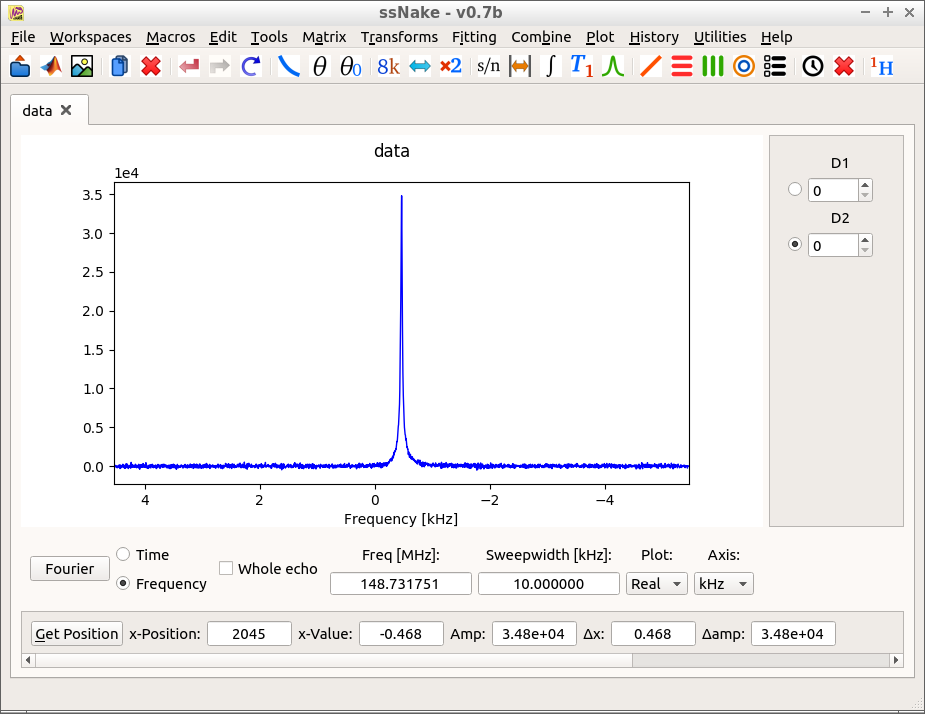
\includegraphics[width=0.8\linewidth]{Figs/Fig1.png}
%\captionof{figure}{Pulse sequence of a single puls enutation experiment.}\label{fig:fig1}
\end{center}


Now we can view the other experiments by increasing the value of the D1 box in the side frame. Note that we want to continue to view the D2 dimension, and therefore keep the bullet next to D2 as the active dimension.

Now we want to examine the change of the peak height along the D1 dimension. We therefore need to get the position of the peak (in data points). Push the `get position' button in the bottom frame, and click on the highest part of the peak (zoom in the be extra accurate). This should print an x-position of approximately  2045. To view this D2 point along D1, copy this value to the D2 box, and push press enter. This gives the following Figure, and shows a sine oscillation with increasing pulse width:
\begin{center}
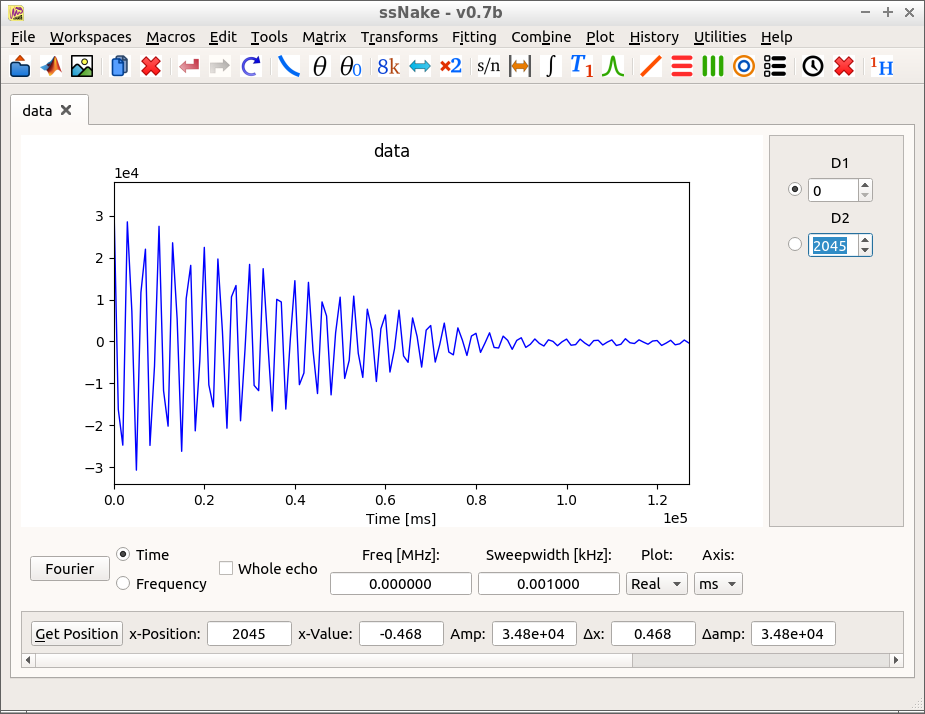
\includegraphics[width=0.8\linewidth]{Figs/Fig2.png}
\end{center}


\begin{itemize}
\item Zero fill along this D1 by using Matrix $\longrightarrow$ Sizing and fill in 1024 points.
\item Right shift the data with 1 point using Matrix $\longrightarrow$ Shift Data, and pushing the right button once. 
\end{itemize}
This gives the following Figure:
\begin{center}
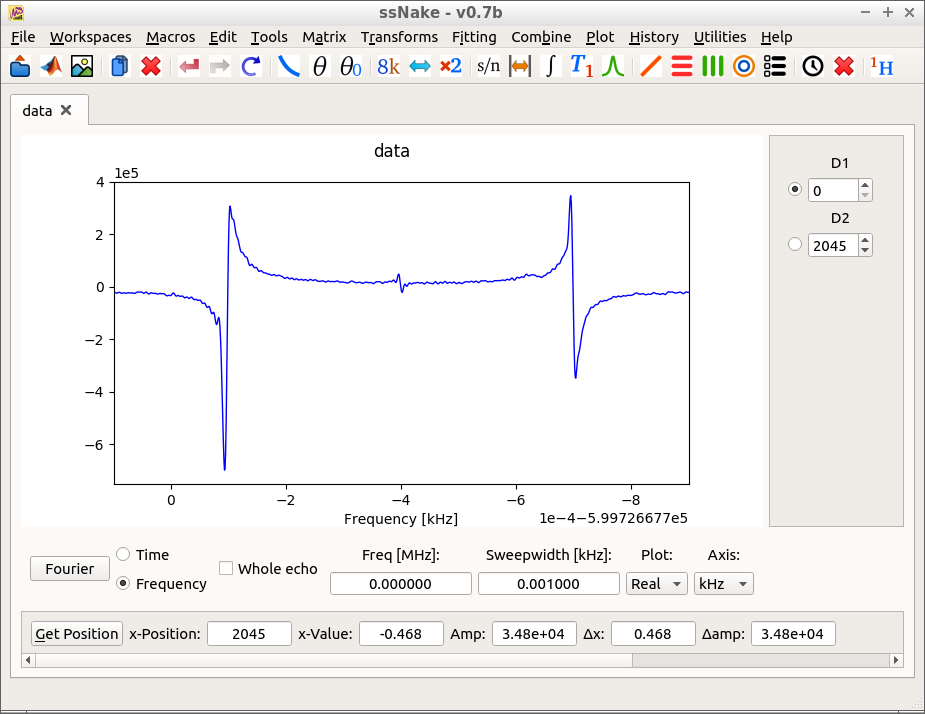
\includegraphics[width=0.8\linewidth]{Figs/Fig3.png}
\end{center}

This last step is removing a data point from the end (in this case an added zero) and puts a zero at the front. This zero represents the spectrum with a pulse width of 0, which we did not measure (but we are sure it gives no signal). This way, we artificially made our oscillation start at $t=0$. 

\begin{itemize}
\item Phase with -90$^\circ$ to get the in-phase spectrum.
\item Clear the reference frequency (none is needed) via Tools $\longrightarrow$ Reference $\longrightarrow$ Clear Current Reference.
\end{itemize}
We now must set the sweepwidth to the right value, as ssNake does not automatically understand what the D1 dimension means. In our case, the dwell time of the experiment is the stepsize of the pulse width: 6~$\muup$s. We can therefore type in the sweepwidth box in the bottomframe: `1000/6e-6'. `1/6e-6' gives us the sweepwidth in Hz, and the 1000 is added for conversion to kHz. Alternatively, `1/6e-3' leads to the same result in a shorter way. This leads to the following Figure, which is the final spectrum. It shows an (nearly) anti-symmetric spectrum with a peak at 50~kHz, so $\nu_1 = 50\;$kHz in this case.
\begin{center}
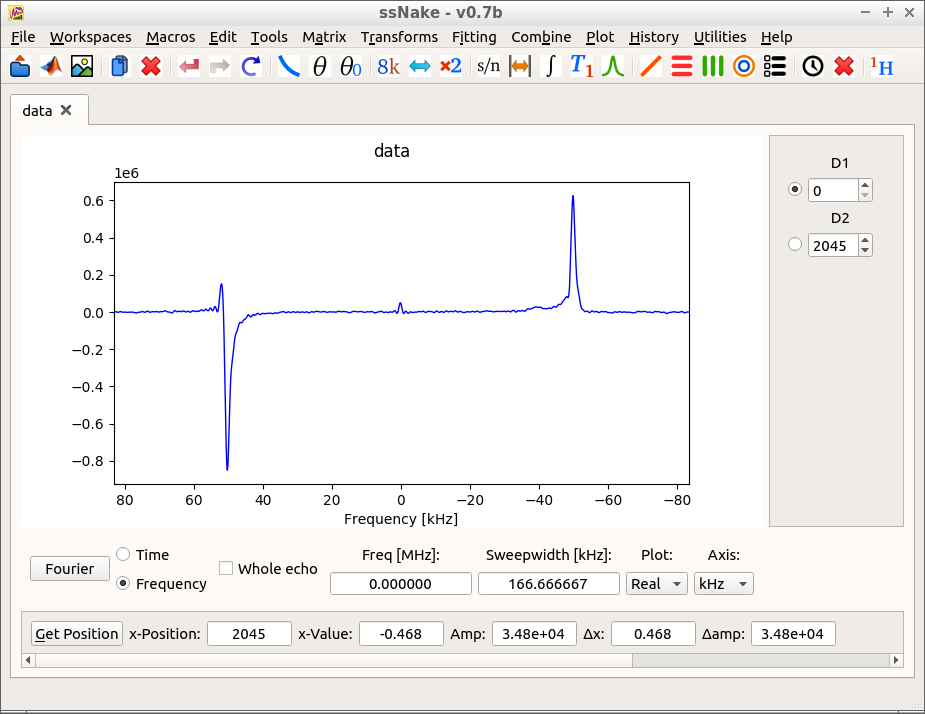
\includegraphics[width=0.8\linewidth]{Figs/Fig4.png}
\end{center}

\section{Alternatives}
\subsection{Integrate D2}
When having phased the first spectrum in D2, Matrix $\longrightarrow$ Region $\longrightarrow$ Integrate can be used to integrate the peak, and get more convenient data. Use the tool by left clicking on the left and right of the peak and press OK. Continue the steps described above, but notice that the old D2 dimension has now been removed, and only the D1 remains. As there is only one dimension now, the dimension selector in the side frame has disappeared. Integrating usually gives a better representation of the nutation spectrum than the via the peak height. This gives the following Figure (after 41.5$^\circ$ 1st order phasing):
\begin{center}
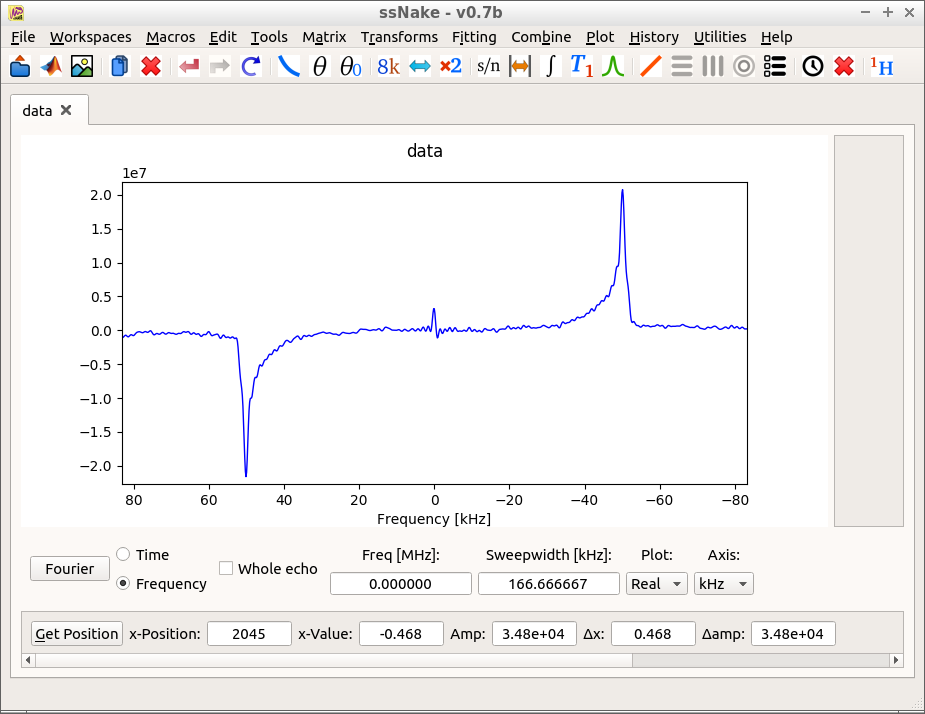
\includegraphics[width=0.8\linewidth]{Figs/Fig5.png}
\end{center}
Note that looks quite different form the `normal' processed spectrum. This probably means that the nutation frequency is not identical over the peak. This is probably caused by bad shimming, which gives a correlation between the NMR frequency (D2) and nutation frequency (D1).



\subsection{Force symmetry}
Ideally, the nutation spectrum has inversion symmetry (the left is -1 times the right). Sometimes it is convenient to force this. This can be done by performing Tools $\longrightarrow$ Real (removing the imaginary part) before the Fourier transform in the D1 domain.

\subsection{Correct DC offset}
In some cases, the nutation signal does not decay to zero, but to some other value. This will give a peak at 0 Hz in the nutation spectrum. This can be avoided by subtracting the average of the last part of the nutation time signal from signal. This can be done by using Tools $\longrightarrow$ Subtract Averages. Ideally, this is done before the zero filling in the D1 domain.

\subsection{2D nutation}
When following the regular method to get the nutation spectrum, the spectrum can be viewed for every point along the D2 dimension, as it is a 2D spectrum. Viewing this can also be done in a contour plot via Plot $\longrightarrow$ Contour.


\end{document}
